\chapter{Einleitung}\label{sec:chapter1}

In der heutigen Zeit sind Softwaresysteme aus dem täglichen Leben nicht mehr weg zu denken \cite{Puntambekar2007}. Diese zeigen bei deren Entwicklung oftmals ein hohes Maß an Komplexität und Umfang auf. Sie müssen nicht nur eine hohe Qualität aufweisen, sondern auch in einer vorgegebenen Zeit zu festgelegten Kosten fertig gestellt werden \cite{Grechenig2010}. Deshalb muss die Entwicklung von Software systematisch durchgeführt werden \cite{gumm2012einfuhrung}. Aus diesem Grund ist es wichtig, bei der Entwicklung eines Systems einem effizienten Softwareentwicklungsprozess zu folgen, da Softwareentwicklungsprozesse den Entwicklungsprozess strukturieren und dadurch beherrschbar machen, indem sie eine Menge von Aktivitäten vorgeben, welche zur Fertigstellung der Software notwendig sind \cite{richling2011autonomie}. Hierbei werden die grundlegenden Aktivitäten bei der Entwicklung eines Softwaresystems wie Planung, Spezifikation, Design, Implementierung und Test strukturiert \cite{gumm2012einfuhrung, Hanser2010}. \newline

Inzwischen existiert eine Reihe verschiedener Softwareentwicklungsprozesse. Diese unterscheiden sich in leichtgewichtige (weniger formal, kaum Dokumentation) und schwergewichtige (sehr formale, dokumentenlastige Vorgehensweise) Prozessmodelle. Scrum ist ein Beispiel für ein leichtgewichtiges Prozessmodell, beim V-Modell XT handelt es sich um ein schwergewichtiges Prozessmodell und der Open Rational Unified Process (Open UP) befindet sich an einer Schnittstelle zwischen schwergewichtigen und leichtgewichtigen Prozessmodellen \cite{Hanser2010}.\newline

Um Softwareentwicklungsprozesse richtig anzuwenden, müssen diese auch verstanden werden. Eine rein textuelle Beschreibung der selbigen ist oftmals sehr umfangreich. Daher sollten diese in einer vereinfachten Art dargestellt werden. Hierfür bieten sich Prozessmodellierungssprachen an, da diese einerseits eine gewisse formale Exaktheit aufweisen und andererseits oftmals auch intuitiv verständlich sind \cite{thomas2009,kircher2006}. \newline

\section{Motivation}



Heutzutage existiert eine Vielzahl unterschiedlicher Prozessmodellierungssprachen. Über deren Vor- und Nachteile wird intensiv diskutiert. Hierbei werden auch sehr häufig die Vorzüge und Nachteile von imperativen und deklarativen Prozessmodellierungssprachen beleuchtet \cite{fahland2010}. \newline

Es gibt bereits Arbeiten und Studien, welche den Vergleich von imperativen und deklarativen Prozessmodellierungssprachen untersuchen. Jedoch gibt es noch kaum Arbeiten, welche sich intensiv mit dem Vergleich der Anwendbarkeit der beiden Prozessmodellierungssprachen bei der Modellierung beschäftigen.\newline

Aus diesem Grund wird die Anwendbarkeit von imperativen und deklarativen Prozessmodellierungsansätzen in dieser Arbeit im Kontext von Softwareentwicklungsprozessen eingehend untersucht werden. Hierfür werden Teile der Softwareentwicklungsprozesse Scrum, Open UP und V-Modell XT sowohl in imperativer als auch in deklarativer Prozessmodellierungssprache modelliert und anschließend wird deren Anwendbarkeit in diesem Kontext analysiert und diskutiert.\newline



\section{Zielstellung}
Die vorliegende Arbeit verfolgt das Ziel, die Anwendbarkeit von deklarativen und imperativen Prozessmodellierungssprachen zu vergleichen. Hierfür soll dem Leser der vorliegenden Arbeit ein grundlegendes Wissen über Software Engineering und Softwareentwicklungsmodelle vermittelt werden. Weiterhin sollen ihm auch grundlegende Kenntnisse in den Bereichen Prozessmodellierung und Prozessmodellierungssprachen, insbesondere imperative und deklarative Prozessmodellierungssprachen beigebracht werden. \newline

Zudem soll eine Einführung des Lesers in die Softwareentwicklungsprozesse Scrum, Open UP und V-Modell XT erfolgen. Das Ziel ist es hier, diese drei Modelle zu analysieren und somit für die nachfolgende Modellierung aufzubereiten.\newline

Ein wichtiges Ziel dieser Arbeit ist es, Teile der Softwareentwicklungsprozesse Scrum, Open UP und V-Modell XT in der imperativen Prozessmodellierungssprache BPMN und in der deklarativen Prozessmodellierungssprache ConDec zu modellieren. Hierdurch wird der Grundstein für den nachfolgenden Vergleich dieser Modelle gelegt.\newline

Das Hauptziel dieser Arbeit ist der Vergleich der Anwendbarkeit der deklarativen und imperativen Prozessmodellierungssprachen. Hierfür werden die zuvor erstellten Modelle genauestens analysiert und die beiden Prozessmodellierungssprachen BPMN und ConDec werden dann bezüglich ihrer Eignung zum Modellieren miteinander verglichen.\newline

Ein weiteres Ziel ist die Validierung des Vergleiches. Die Validierung wird mit Hilfe einer Studie durchgeführt, bei welcher mehrere Studierende und Doktoranden der Informatik befragt werden.\newline





\section{Aufbau der Arbeit}

Eine Übersicht über den Aufbau dieser Arbeit gibt Abbildung \ref{fig:Aufbau}.
Zunächst werden in Kapitel 2 und 3 grundlegende Begriffe erläutert, welche für das Verständnis der vorliegenden Arbeit notwendig sind.\newline

Kapitel 2 liefert einen Einblick in Prozessmodelle. In Kapitel 2.1 wird der Begriff Software Engineering eingeführt. Anschließend werden in Kapitel 2.2 Softwareprozesse erläutert. Hierfür werden Software-Projekttypen sowie schwergewichtige und leichtgewichtige Prozessmodelle definiert.\newline

In Kapitel 3 erfolgt eine Einführung in die Grundlagen der Modellierung. Zum einen werden in Kapitel 3.1 Prozessmodellierung, die Ziele der Prozessmodellierung sowie die Grundsätze ordnungsgemäßer Modellierung vorgestellt. Zum anderen erfolgt in Kapitel 3.2 eine allgemeine Einführung in Prozessmodellierungssprachen und vor allem werden die in dieser Arbeit verwendete imperative und deklarative Modellierung erklärt. Des Weiteren werden noch in Kapitel 3.3 die in der vorliegenden Arbeit verwendeten Modellierungswerkzeuge beschrieben.\newline

Die Anforderungserhebung erfolgt in Kapitel 4. Hier werden in Kapitel 4.1 die Vergleichskriterien für die beiden Prozessmodellierungssprachen erläutert.\newline

Die imperative und deklarative Modellierung für Software Engineering Prozessmodelle erfolgt in Kapitel 5. Es wird das Software Engineering Prozessmodell Scrum in Kapitel 5.1 zunächst eingeführt, anschließend analysiert, imperativ und deklarativ modelliert und die imperativen und deklarativen Modellierungen werden miteinander verglichen. In Kapitel 5.2 wird dann der Open Unified Process (Open UP) vorgestellt, es folgt eine Analyse des selbigen und es werden imperative und deklarative Modelle des Open UP erstellt und miteinander verglichen. Das V-Modell XT wird in Kapitel 5.3 erläutert, analysiert, imperativ und deklarativ modelliert und die jeweiligen Modelle werden einander gegenüber gestellt. In Kapitel 5.4 erfolgt ein übergreifender Vergleich der imperativen und deklarativen Modelle.\newline

Die Validierung der Ergebnisse aus Kapitel 5 wird in Kapitel 6 durchgeführt. Zunächst werden in Kapitel 6.1 die Forschungsfragen vorgestellt. Anschließend wird in Kapitel 6.2 das Design der Studie erklärt und es wird in Kapitel 6.3 die Durchführung der Studie erläutert. Abschließend erfolgt in Kapitel 6.4 ein Fazit der Studie.  \newline

Kapitel 7 widmet sich verwandten Arbeiten zur vorliegenden Arbeit. Zunächst werden in Kapitel 7.1 verwandte Arbeiten zur Modellierung von Software Engineering Prozessmodellen gegenüber der vorliegenden Arbeit abgegrenzt. Weiterhin werden in Kapitel 7.2 Arbeiten über die Verständlichkeit von Prozessmodellierungssprachen und in Kapitel 7.3 Arbeiten über den Vergleich von Prozessmodellierungssprachen dargelegt und der Thematik dieser Arbeit gegenüber gestellt.\newline

Kapitel 8 fasst die gesamte Arbeit nochmals zusammen und gibt einen Ausblick auf zukünftige Forschung in dieser Thematik.

\begin{figure}[htp]
\begin{center}
  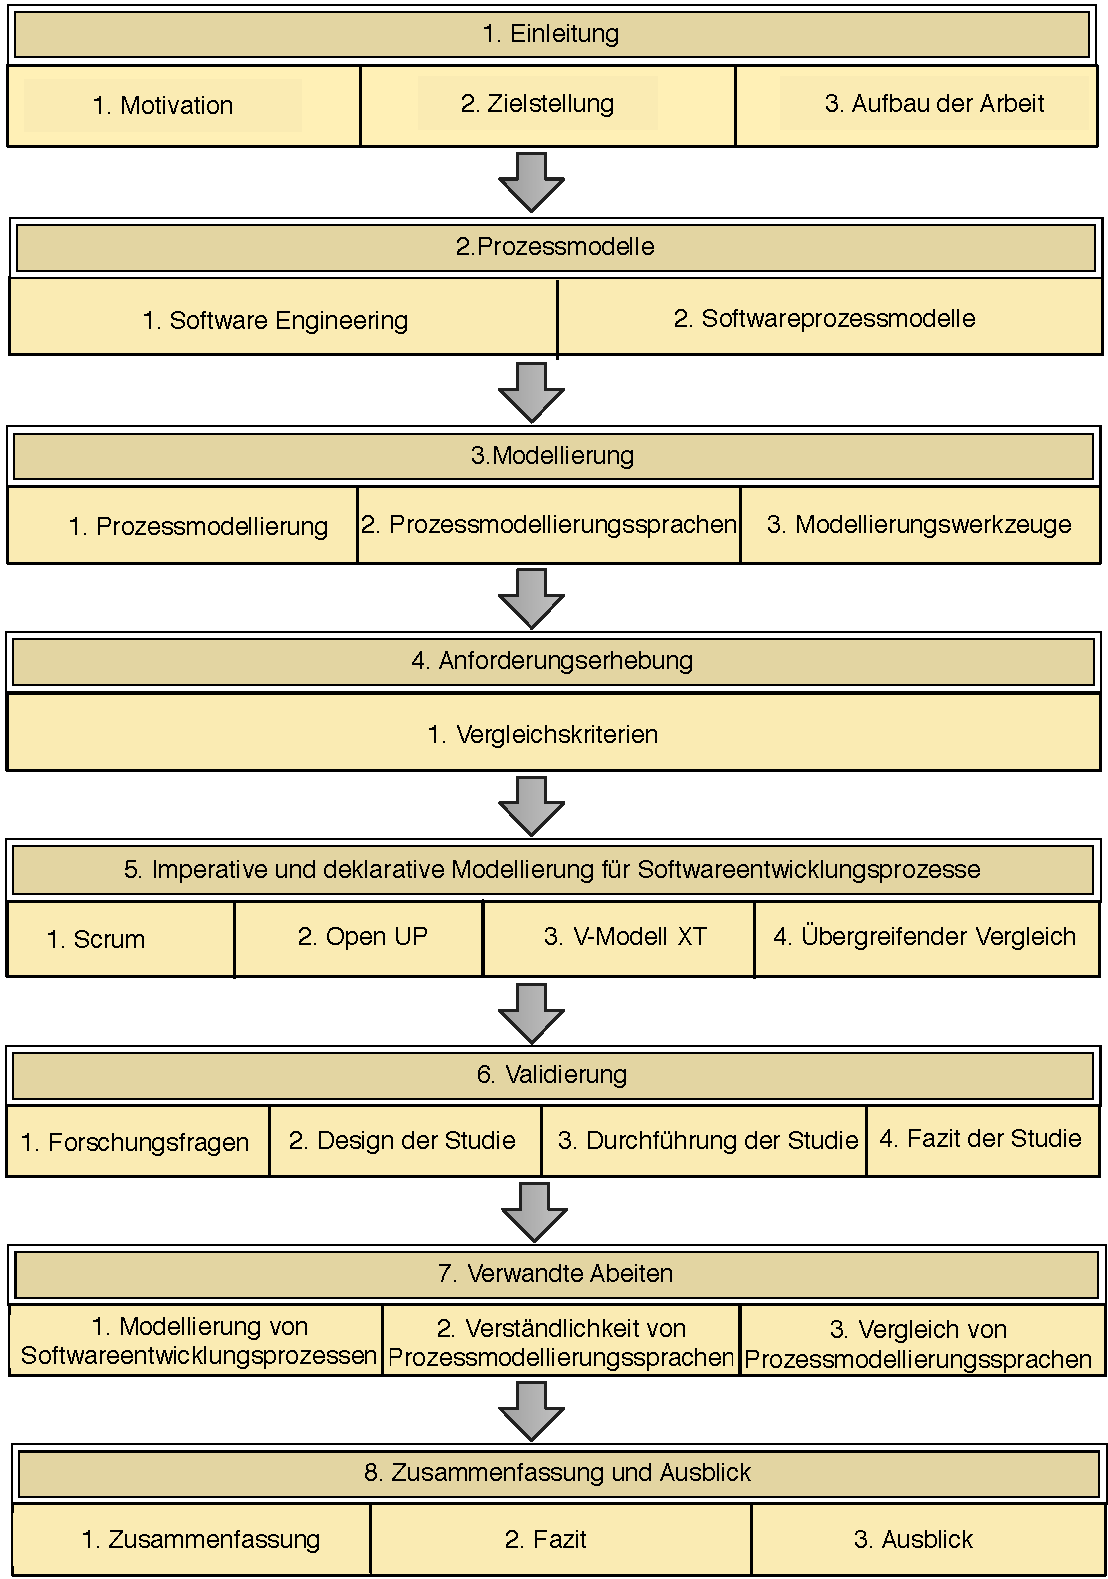
\includegraphics[scale=0.8]{Aufbau} %pdf, jpg, png...
  \caption{Aufbau der Arbeit}
  \label{fig:Aufbau}
\end{center}
\end{figure}

